%%%%%%%%%%%%%%%%%%%%%%%%%%%%%%%%%%%%%%%%%%%%%%%%%%%%%%%%%%
\section{\label{app:D:HalfmodeThreshold}Robustness of the halfmode analysis}
%%%%%%%%%%%%%%%%%%%%%%%%%%%%%%%%%%%%%%%%%%%%%%%%%%%%%%%%%%
\renewcommand{\theequation}{D-\arabic{equation}}
% redefine the command that creates the equation no.
\setcounter{equation}{0}  % reset counter 

\begin{figure}[ht]
\begin{tabular}{lr}\hspace{-1cm}
 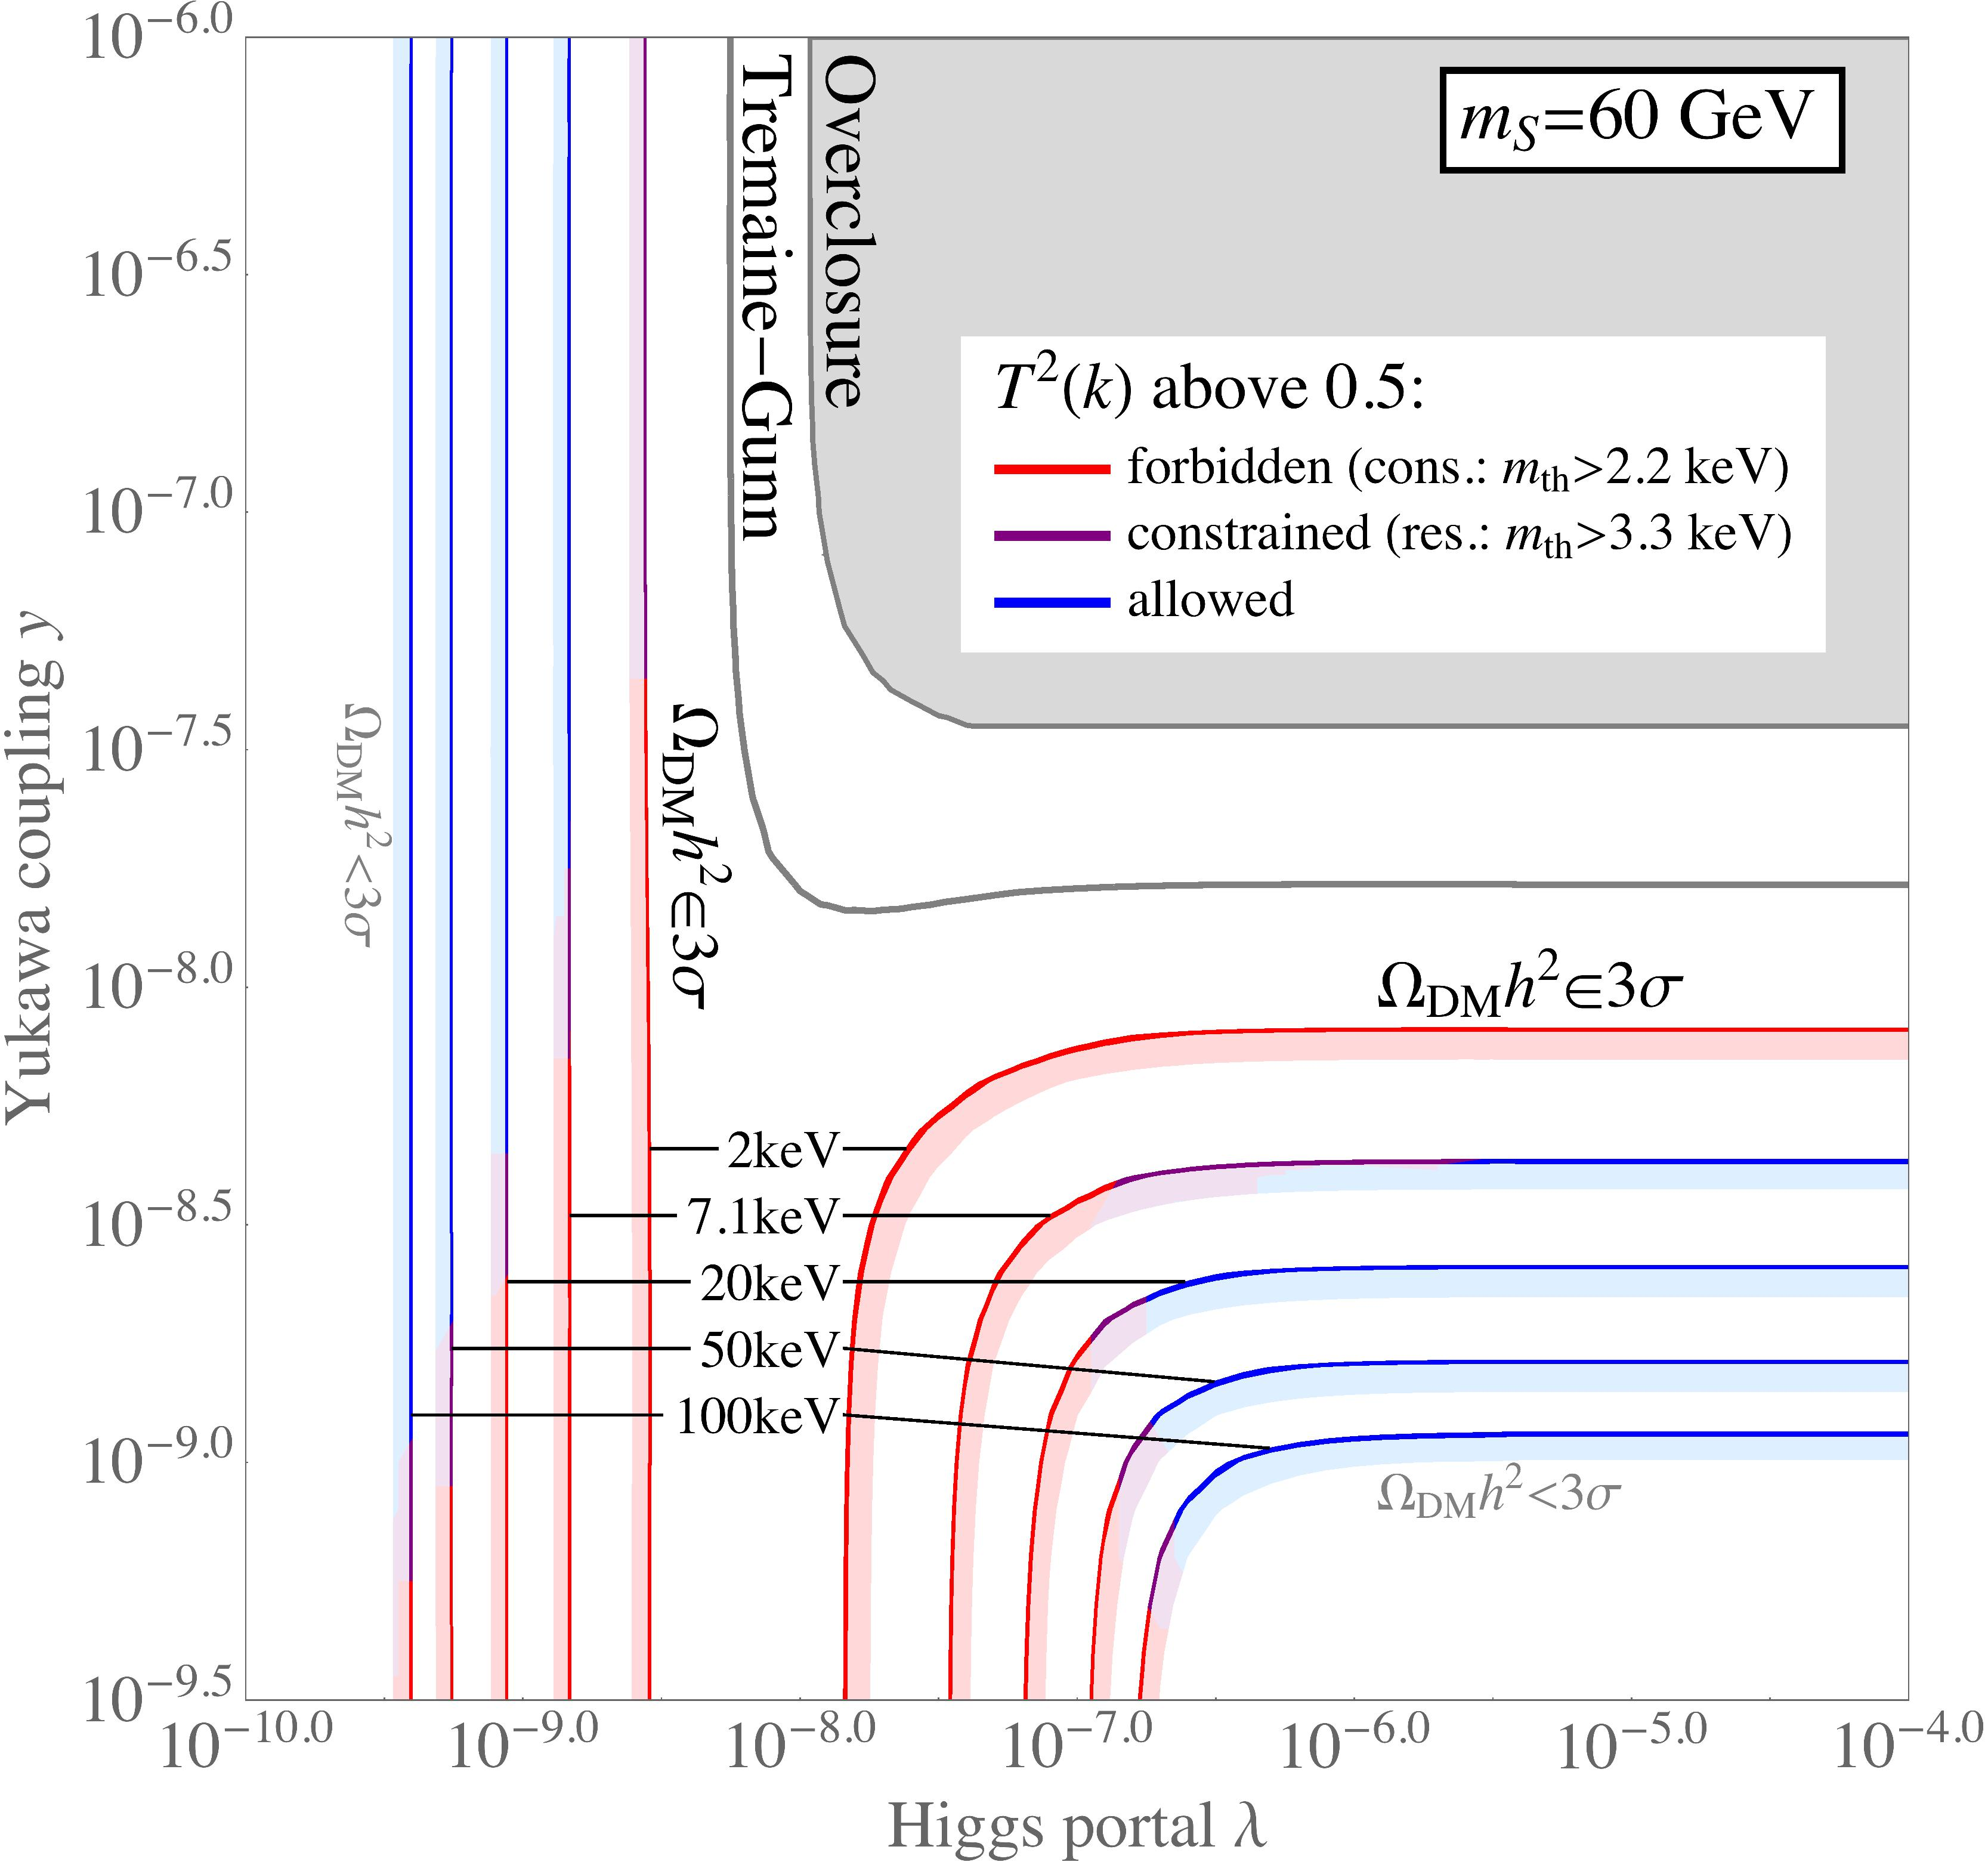
\includegraphics[width=8.3cm]{figures/HalfMode_60_until4_relpower0p5.jpeg} & 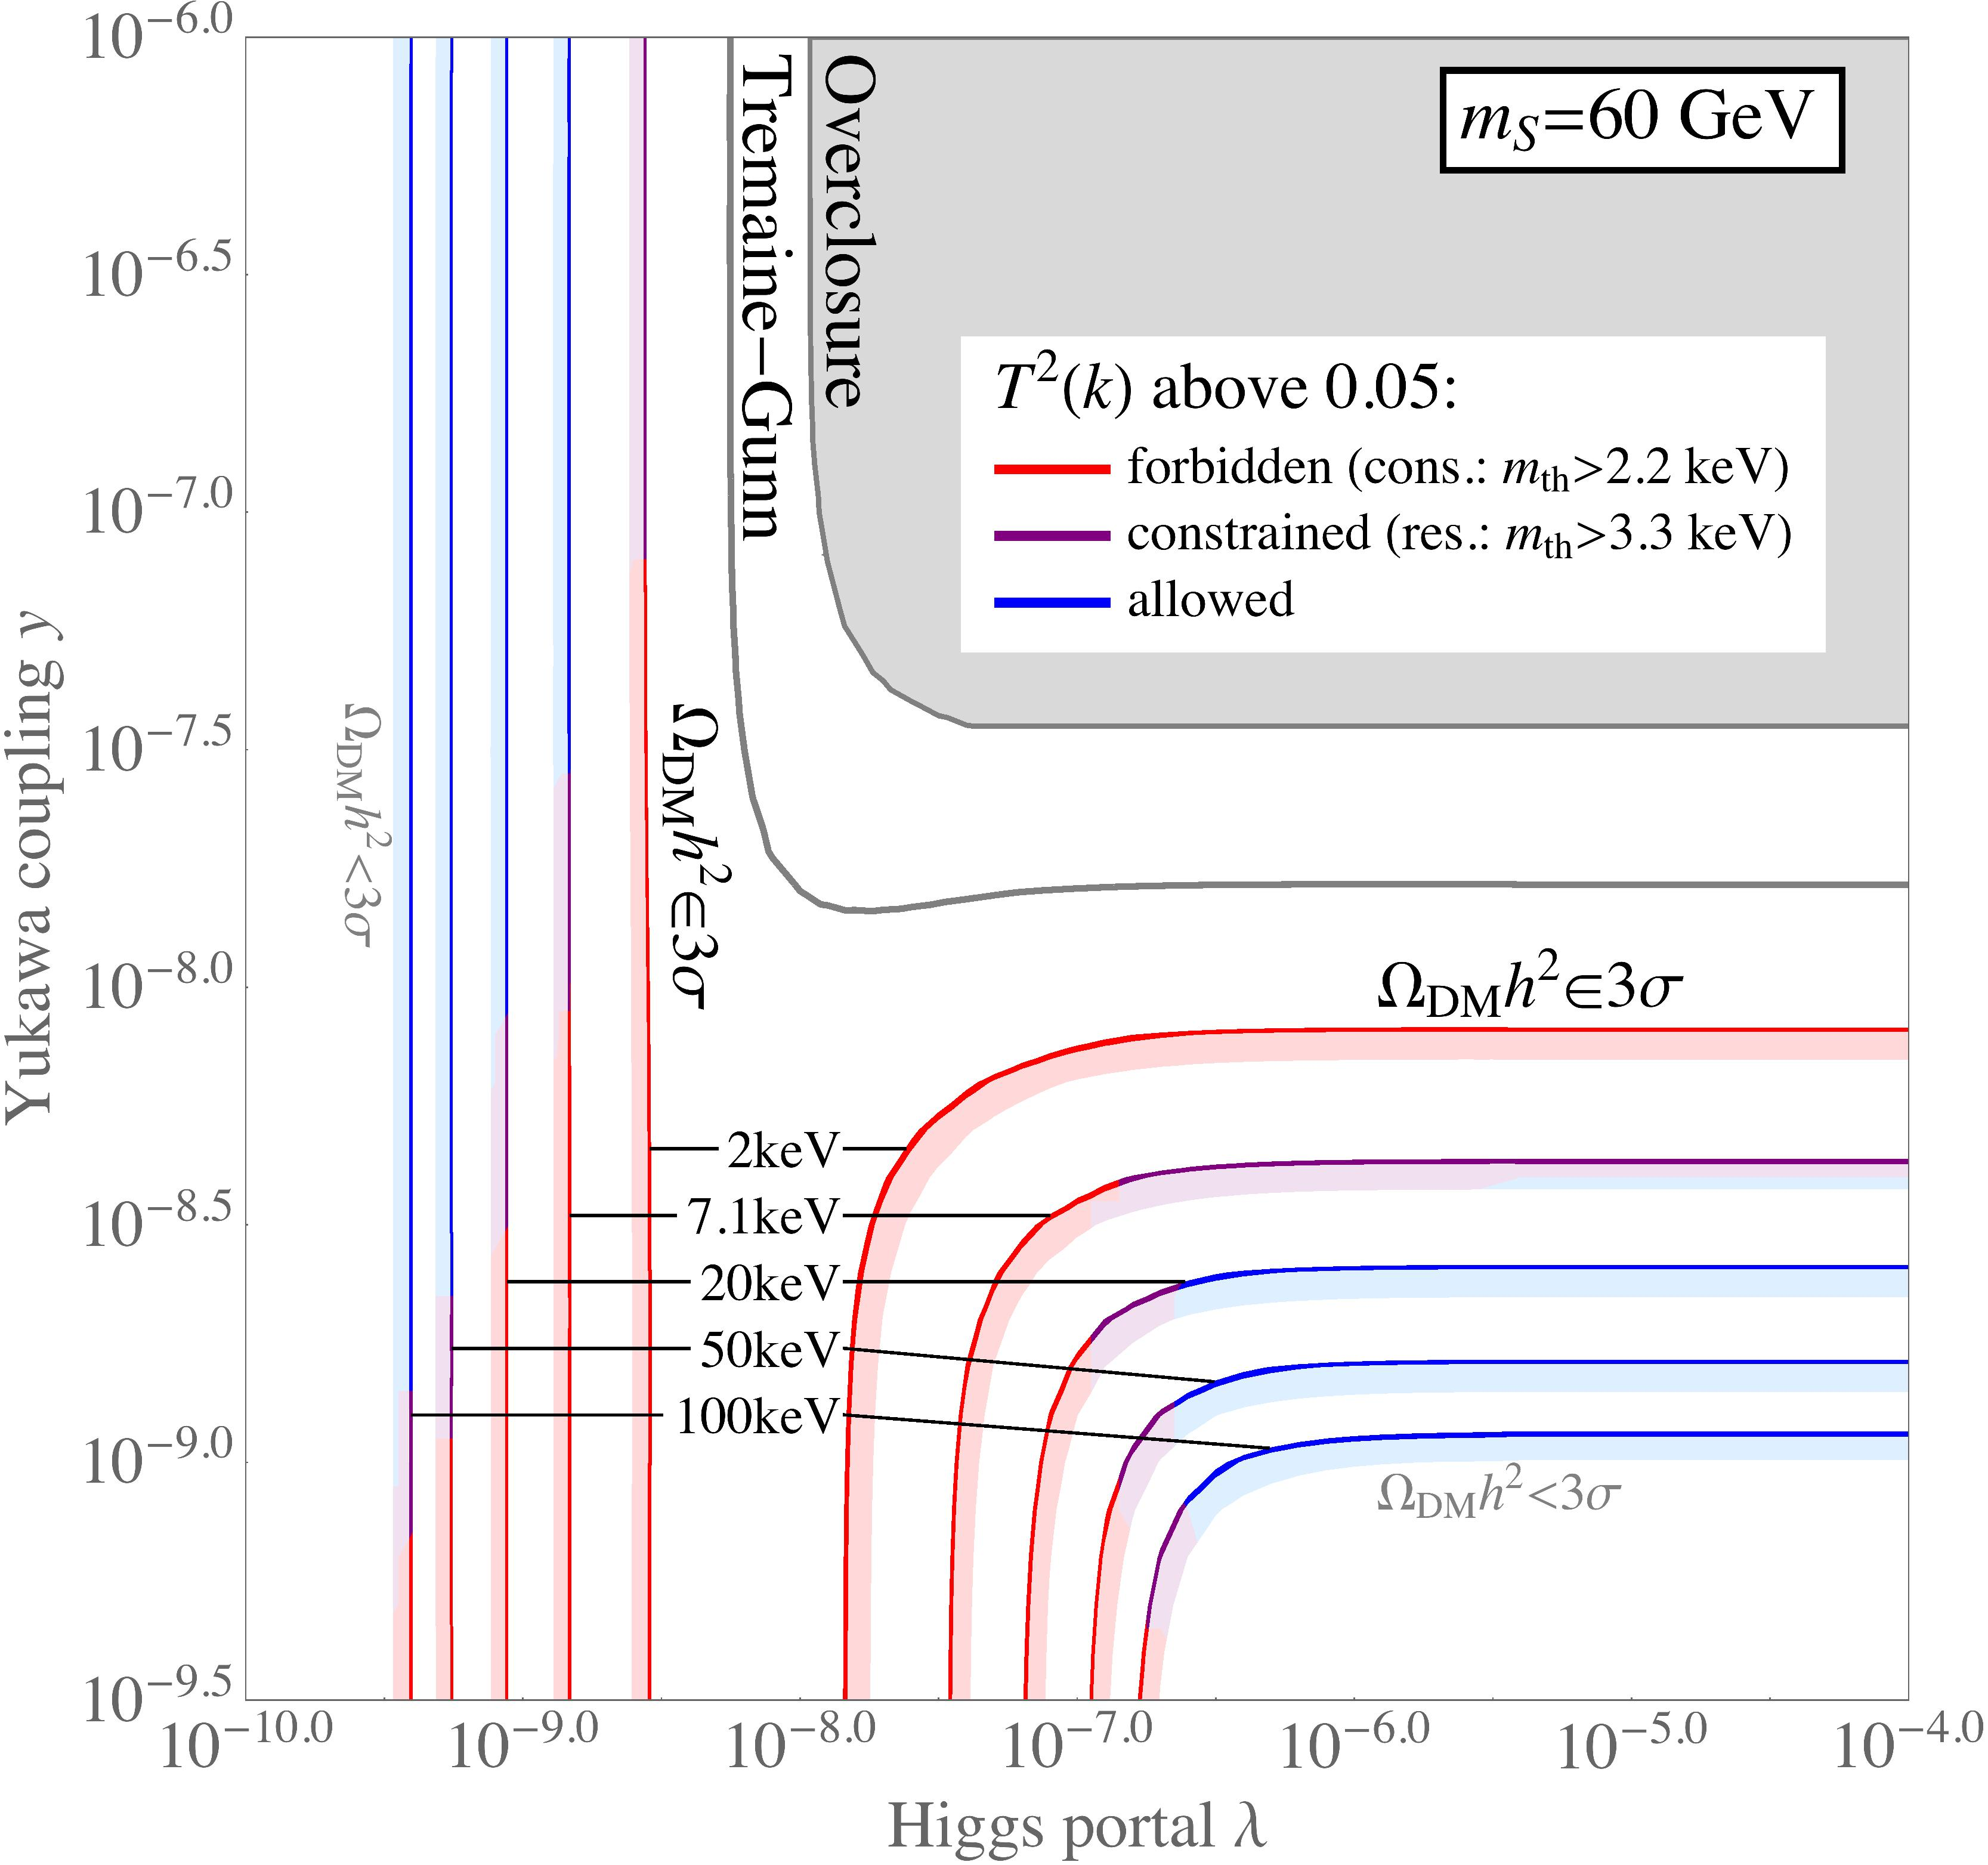
\includegraphics[width=8.3cm]{figures/HalfMode_60_until4_relpower0p05.jpeg}
\end{tabular}
\caption{\label{fig:HalfmodeThreshold}Compatability of the scalar decay model with $m_S=\unit{60}{GeV}$ for different threshold wave numbers. The \emph{left} panel contains the analysis with $k_x=k_{1/2}$ (as used throughout Sec.~\ref{sec:Results}; the plot displayed here is basically identical to the right Fig.~\ref{fig:verysmall_masses}, except for the model-dependent bounds not being displayed to enable a better comparison), while the \emph{right} panel displays $k_x= k_{0.05}$. The comparison shows that the changes are minor, but they will be finally specified in an upcoming work of us aiming to compared several advances methods to derive bounds from structure formation.}
\end{figure}

At first sight, the definition of the halfmode in \equref{eq:Def:Half-mode} might seem just as arbitrary as the free-streaming boundary between ``cold'' and ``warm'' (``warm'' and ``hot'') at $\unit{0.01}{Mpc}$ ($\unit{0.1}{Mpc}$). Even though the transfer function falls off steeply around $k_{1/2}$, it is a priori unclear at which value of the squared transfer function the discrimination becomes indeed negligible. While a more fundamental analysis of structure formation (e.g.~by rederiving Lyman-$\alpha$ bounds for non-thermal spectra) is beyond the scope of this paper and is projected for future work, we can nonetheless test the robustness of our analysis against changes in the threshold given in \equref{eq:Def:Half-mode}. More specifically, we can make our analysis more restrictive by comparing not only wavenumbers smaller than $k_{1/2}$ but wavenumbers smaller than some $k_x$ with $x < 0.5$, which translates to $k_{1/2} < k_x$. In order to demsonstrate that the analysis is rather robust even against large changes in this threshold, we have reanalysed the case of a scalar with $m_S = \unit{60}{GeV}$ with a $k_x=k_{0.05}$. \Figref{fig:HalfmodeThreshold} shows that even this rather drastic change in the threshold power (by one whole order of magnitude) inflicts rather mild changes on the results. This would be dramatically different when changing the values put in as boundaries in a free-streaming analysis (cf.~\Figref{fig:FS-comparison}). 

Even though being approximate itself, our method of incorporating bounds from structure formation, using Lyman-$\alpha$ data derived for thermal spectra, clearly proves more reliable than the free-streaming approach.